\documentclass[twoside,leqno, 11pt]{article}  
%twocolumn
\usepackage{ltexpprt} 
\usepackage{url}
\usepackage{framed}
\usepackage{amsmath}
\usepackage{authblk}
\usepackage{cite}
\usepackage{verbatim}
\usepackage{graphicx}
\begin{document}
\title{\Large  Joint Optimization of Routing and Node Selection}
%\thanks{Supported by .} 
\author[]{Moses Charikar}
\author[]{Yonatan Naamad}
\author[]{Jennifer Rexford}
\author[]{Kelvin Zou}
\affil[]{Department of Computer Science, Princeton University}
\affil[ ]{\textit {\{moses,ynaamad,jrex, xuanz\}@cs.princeton.edu}}
\date{}

\maketitle
%%%%%%%%%%%%%%%%%%%%%%%%%%%%%%%%%%%%%
%%%%%%%%%%                         Abstract                                 %%%%%
%%%%%%%%%%%%%%%%%%%%%%%%%%%%%%%%%%%%%
\begin{comment}
\begin{abstract} \small\baselineskip=9pt This is the text of my abstract. It is a brief
description of my
paper, outlining the purposes and goals I am trying to address.\end{abstract}
\end{comment}

%%%%%%%%%%%%%%%%%%%%%%%%%%%%%%%%%%%%%
%%%%%%%%%%                         Intro                                 %%%%%
%%%%%%%%%%%%%%%%%%%%%%%%%%%%%%%%%%%%%

 \section{Problem formulation} In this paper, we introduce a network flow model. If we review the network abstraction, it is essentially composed of nodes, links and flows. However the model is missing one important piece for networking. Network flows are not simply just like water, a lot of processing work are carried via flows and need to be done before the flow reaches destination. What if flow needs to be processed at some node along the path? What is more interesting is that due to the fact that each node has a certain processing capacity, we cannot actually handle the flow at a single node, but instead they are handled at different nodes, saying we can handle half at the first hop and the other half at the second node. This essentially leads to an interesting graph model: we have a graph G(V, E), with both link bandwidth \textbf{B}(e)where $e \in E(u,v)$ and node capacity \textbf{C}(v)where $v \in V $, and we are trying to fill in traffic demand with both traffic rate demand \textbf{R}(src, dest) and computational work demand \textbf{D}(src, dest). \textbf{R}(src, dest) should be correlated to \textbf{D}(src, dest). Throughout the whole paper, we assume linear relation $q_i = \frac{D}{R}$ for each flow $ i_{src,dst} $right now, which covers most cases, since most workload processing is per packet based. The system can achieve a joint optimal outcome for both routing and node workload allocation usage by coupling routing problem to processing resource placement and processing resource allocation problem.  
 
\textbf{Hard Constraints}:
\newline
\textbf{B}(e): bandwidth capacity for link e $\in E_{u,v}$
 \newline
\textbf{C}(v): middlebox processing capacity at node v $\in N_{v}$
 \newline
$ \boldsymbol{R}_{i} \text{: flow rate R for } i_{src, dst}$ 
\newline
$ \boldsymbol{D}_{i} \text{: flow middlebox processing demand for } i_{src, dst}$
\newline 
$ q_{i} \text{: ratio of D to R for flow } i_{src, dst}$ 
%%%%%%%%%%%%%%%%%%%%%%%%%%%%%%%%%%%%%
%%%%%%%%%%%%%%%%%%%%%%%%%%%%%%%%%%%%%
%%%%%%%%%%                         Max flow model                         %%%
%%%%%%%%%%%%%%%%%%%%%%%%%%%%%%%%%%%%%
\section{Max Flow Model}
\subsection{Edge-based formulation}To help us understand the problem, we need to simplify the model, instead of focus on multiple commodity flows, we only focus on one flow with single source and single destination, and ask the basic question: what is the maximum amount of flow along with its processing demand being processed and sent to destination given a graph with a certain node capacity and link capacity for each node and link. Without losing generality and to make the math easier to read, we assume ratio between workload and flow size is 1, i.e. one flow requires one unit of processing. We also assume it is undirected graph as it is closer to real networking setting. %citation needed.

\textbf{Notations:}

B(e): bandwidth capacity for link $e \in E$,

C(v): middlebox processing capacity at node $v \in V$,

$ f(e): $  flow load at edge $e\in E $, 

$ w(e):$ workload demand at edge e, 

$p(v): $   workload processed at node v,

$p(v) = \sum\limits_{in } w(e) - \sum\limits_{out} w(e)  $. 
 
 At the first glance, this problem looks like Max flow problem, however the reduction does not work quite well, to help us better understand the problem, we can formulate it in a general purpose LP to get better insight.
%%%%%%%%%%%%%%%%%%%%%First LP%%%%%%%%%%%%%%%%%%%%%%%

Objective: Maximize $\sum \limits_{e=(s, v) \in E} f(e) $

Subject to:
\begin{subequations}
\begin{align}
&\forall v \in V-\{s, t\}; \sum\limits_{in}  f(e)= \sum\limits_{out} f(e),\\
&\forall e; f(e)\geq 0,\\
&\forall e; f(e)\leq B(e),\\
&\forall e; w(e) \geq 0,\\
&\forall e; w(e) \leq f(e),\\
&\forall v; p(v) = \sum\limits_{in } w(e) - \sum\limits_{out} w(e),\\
&\forall v; p_v\geq 0 ,\\
&\forall v; p_v\leq C(v),\\
&\forall e\in(s, v) ; w(e) =f(e),\\
&\forall e\in(v,t) ; w(e) =0.
\end{align}
\end{subequations}
  
If we look closely into the correlation between w and f, here we have (2.1e) which is saying every time workload can only be carried out by flow, so it should be less than or equal to flow size. There is an alternative way to interpret this problem with just flows, that is we have two types of flows, pre-processed and post-processed, here we denote $f^1$ as pre processed, and $f^2$ as post processed. Flows are dynamically changing according to workload processed at each node; where $f^1$ is decreasing and $f^2$ increasing as flow routed from source to destination, . 
%%%%%%%%%%%%%%%%%%%%%Second LP%%%%%%%%%%%%%%%%%%%%%%%

Objective: Maximize $\sum \limits_{v: (s, v) \in E} f^1(e) $ 

Subject to:
\begin{subequations}
\begin{align}
&\sum\limits_{in} ( f^2(e)+ f^1(e))= \sum\limits_{out } ( f^2(e)+ f^1(e))\\
&for\; \forall v \in V-\{s, t\}; \nonumber\\
&\forall e; f^2(e)\geq 0,\\
&\forall e; f^1(e)\geq 0,\\
&\forall e; f^1(e)+ f^2(e)\leq B(e),\\
&\forall v; p(v) = \sum\limits_{in } f^1(e) - \sum\limits_{out} f^1(e) \\
&\forall v;p(v)\geq 0, \\
&\forall v;p(v)\leq C(v),\\
&\forall e\in (s,v); f^2=0, \\
&\forall e\in (v,t); f^1=0,
\end{align}
\end{subequations}

Understanding the LP: so in this linear programming model $f^1 $ is essentially w for the LP 2.1, and $f^2 = f-w$ essentially. The advantages here may not be obvious, but it would help understand the structure of the problem and also easier to adapt for more advanced requirement in formulation.%somesection.

\subsection{Path-based formulation}
Unlike edge-based solution, which is not so intuitive and require proof for feasibility, path based solution is correct by design. Here we also formulate a path based Linear Programming model and later show the equivalence between them.
In this section we are formulating in f/w representation. Here we have f($\pi$) which represents the flow for each path, and p($\pi$, e) represents the workload processed at node v of each edge (u,v).

Objective: Maximize  $\sum \limits_{\pi\in P} f(\pi) $

Subject to:
\begin{subequations}
\begin{align}
&\forall e; \sum \limits_{\pi\in P:e\in \pi} f(\pi) \leq B(e),\\
&\forall \pi; \sum \limits_{e\in \pi} p(\pi, e) = f(\pi),\\
&\forall  v; \sum \limits_{\pi\in P} \sum \limits_{ e\equiv (u,v)\in \pi} p(\pi, e) \leq C(v),\\
&\forall e; f(e)\geq 0, \\
&\forall \pi, e; p(\pi,e) \geq 0,
\end{align}
\end{subequations}

%%%%%%%%Comment out part%%%%%%%%%%%%%%%

\begin{comment}
[$f^1/f^2$] Optimization Objective:
\newline

Maximize  $\sum \limits_{\pi\in P} f(\pi) $
\newline

Subject to:
\newline
\begin{subequations}
\begin{align}
&\forall e, \pi;  f^1(\pi, e) +f^2(\pi, e) = f(\pi),\\
&\forall e; \sum \limits_{\pi\in P:e\in \pi} f(\pi) \leq B(e),\\
&\forall  v; \sum \limits_{\pi\in P} \sum \limits_{ e,e'= (u,v,w)\in \pi} f^2(\pi, e') -f^2(\pi, e)\leq C(v),\\
&\forall e; f^2(\pi,e)\geq 0, \\
&\forall e; f^1(\pi,e)\geq 0, \\
&f^2(\pi,(s,v))= 0, \\
&f^1(\pi, (w,y)) =0, 
\end{align}
\end{subequations}
\end{comment}

%%%%%%%%Comment out part%%%%%%%%%%%%%%%


%%%%%%%%%%%%%%%%%%%%%%%%%%%%%%%%%%%%%%%%
%%%%%%%%%%%%%%%%%%%%%%%%%%%%%%%%%%%%%%%%
%%%%%%%%%%%                     Dual LP              %%%%%%%%%%%%%%
%%%%%%%%%%%%%%%%%%%%%%%%%%%%%%%%%%%%%%%%
%%%%%%%%%%%%%%%%%%%%%%%%%%%%%%%%%%%%%%%%

The dual LP for the path based solution:

Objective: Minimize $\sum \limits_{e \in E} B(e)* X_e +\sum \limits_{v \in V} C(v)*Y_v $

Subject to:
\begin{subequations}
\begin{align}
&\forall \pi \in P \; \&\; \forall v \in \pi; \sum \limits_{e\in \pi} X_e + Y_v \geq 1,\\
&\forall e \in E; X_e\geq 0,\\
&\forall v \in V; Y_v\geq 0.
\end{align}
\end{subequations}

To help understand the relation between $p(\pi, e)$ and $f(\pi)$, again we introduce two intermediate variables, $f^1(\pi, e), f^2(\pi, e) $ represents respectively pre processed and post processed flow at edge e on the path $\pi$, so $f^2(\pi, e) =\sum\limits_{e'\; before\;e}p(\pi, e') $ and $ f^1(\pi, e)=f(\pi)- f^2(\pi, e)$, it is not hard to see that $f^2$ is topologically increasing while $f^1$ is topologically decreasing.



%%%%%%%%%%%%%%%%%%%%%%%%%%%%%%%%%%%%%%%%
%%%%%%                            first definition                       %%%%%%%%%%%
%%%%%%%%%%%%%%%%%%%%%%%%%%%%%%%%%%%%%%%%
\begin{Definition}
Simple path: if there is(are) cycle(s), it has ingress $f^2 = 0$ and egress $f^1=0$ for all cross points for each cycle. 
\end{Definition}

\begin{lemma} If there is a cycle in the path composition, we can achieve in the cycle there are two different edges where one has $min(f^2) = 0$ and one has $min(f^1)=0$. 
\end{lemma}

\begin{proof} it is similar to flow cancellation in a simpler graph model without workload: 

1. for e=(u,v) whereas $min(f^1) >0$, we can simply cancel the unprocessed flow demand by small amount $\epsilon$, and it does not affect the outcome of the flow outside the loop, while we can reduce the flow load and workload demand in the loop without side effect. 

2. for e=(u,v) whereas $min(f^2)>0$, we can cancel the processed flow demand by small amount $\epsilon$, and this does not affect the outcome of the flow outside of the loop while we can reduce the flow load in the loop without side effect. 


The intuition behind this is that loop exists due to that some flow needs to borrow some processing capacity from some node(s), so it would "detour" a flow with fully unprocessed workload and get back the flow with fully processed workload. 
\end{proof}

\begin{lemma} If there is a cycle in a path, $f^2_{min}= 1$ and $f^1_{min} = 0$ are at the the some node and the node is cross point. 
\end{lemma}
\begin{proof}
we apply lemma2.1: there must be one edges in the cycle where $f^1$=0. Since for the path, we have $f^1$ decreasing along the path, so at some node in the cycle we have $f^1_{n, n'}=0$, then we can follow the w value traverse downstream, until we reach the exit edge pointing to cross point, it also have  $f^1_{crossPoint\_out}=0$. 

Use the same mechanism, we can prove that $f^2_{crossPoint\_in}=1$. Since we have flow conservation, so f is the same along the path. Meanwhile we have at some node n where $f^2_{n,n'}=0$, and if we traverse upstream we will encounter the entering node pointing from cross point, where we still have $f^2=0$, since $f^2$ is increasing along the path.
\end{proof}

\begin{lemma} If a cycle only between two nodes, then we have two reversed flows with one $f^1=0$ and the other $f^2=0$.
\end{lemma}
This is a simple extension from lemma2.2, since we only have two edges in the cycle, and one must be incoming edge and the other outgoing edge. 

%%%%%%%%%%%%%%%%%%%%%%%%%%%%%%%%%%%%%%%%
%%%%%%                            Algorithm part?                      %%%%%%%%%%%
%%%%%%%%%%%%%%%%%%%%%%%%%%%%%%%%%%%%%%%%
\section{Algorithm}
One thing makes this problem significantly harder than simple Max Flow is that it violates several key assumptions in Max flow: 1. in max flow we only select simple paths, while here cycles are valid; 2. in max flow if you have f(u,v)= -f(v,u), and here you could have f(u,v) and f(v,u) both positive. 

If we look closely to the problem, there are two directions to solve these problems: either model this as a circulation or two-flow problem. We choose two flow model since circulation problem does not do well in handling several cycle. 

So here is the modeling:\newline
 We can think it as multiple commodity flows, and $f^1$ is heading from source to some node v, and $f^2$ is going out from node v to destination. Here we have $f^1=f^2$ for all nodes.  





%%%%%%%%%%%%%%%%%%%%%%%%%%%%%%%%%%%%%%%%
%%%%%%                            Flow size change                    %%%%%%%%%%%
%%%%%%%%%%%%%%%%%%%%%%%%%%%%%%%%%%%%%%%%
\section{Flow Size Change after Processing}
The model above shows the model where workload processing does not affect the traffic size. However this is not always the case in networking setting, for example, encryption increase the flow size by a little bit via changing either the header or both header and payload\cite{SIMPLE2013}; compression and transcoding decrease the traffic size by up to a factor of two\cite{Mogul1997}. We need to also put this into our optimization formulation.

There have been some work done regarding flow size change in max flow problems, so called generalized circulation max flow problem.\emph{Wayne, 1999}\cite{Wayne1999}  One thing different in our model is that flow size change does not apply for all flows. For pre processed flow handled at that node, the size would be changed, but for post processed flow, it stays the same. So here we need to make some change from the previous LP to make the expression more succinct. 
Again we divide the flow into two categories; pre-processed, and post-processed. They are represented in $f^1$ and $f^2$ respectively. 

If there is a size change, at each node, we have $\sum\limits_{in} f^1(e) - \sum\limits_{out}  f^1(e) = p(v)$ and $\sum\limits_{out} f^2(e)-\sum\limits_{in}  f^2(e) = p(v)*r; r>0$. (We assume the linear relation between flow size, which satisfy most networking settings). However this way we would violate the flow conservation, that is incoming flow size does not match outgoing flow size anymore. [See appendix for proof of the LP]

Objective: Maximize $\sum \limits_{v: (s, v) \in E} f^1(e) $

Subject to:
\begin{subequations}
\begin{align}
& [\sum\limits_{out}  f^2(e) -\sum\limits_{in} f^2(e)]*r= \sum\limits_{in } f^1(e)-  \sum\limits_{out }  f^1(e) 
\end{align}
\begin{align}
&for\; \forall v \in V-\{s, t\};\nonumber\\
&\forall e; f^2(e)\geq 0\\
&\forall e; f^1(e) \geq 0\\
&\forall e; f^2(e) + f^1(e)\leq B(e)\\
&\forall v; p(v) = \sum\limits_{in } f^1(e) - \sum\limits_{out} f^1(e) \\
&\forall v;p(v)\geq 0 \\
&\forall v;p(v)\leq C(v)\\
&\forall e\in (s,v); f^2=0\\
&\forall e\in (v,t); f^1=0
\end{align}
\end{subequations}

%%%%%%%%%%%%%%%%%%%%%%%%%%%%%%%%%%%%%%%%%%%%%%%%%%%
%%%%%%%%%                      Multi tasks for a flow                     %%%%%%%%%%%%%%%%%%
%%%%%%%%%%%%%%%%%%%%%%%%%%%%%%%%%%%%%%%%%%%%%%%%%%%
\section{Multiple Tasks for a flow}
In real network, usually a flow needs to go through several different processes before reaching destination. So far we assume the nodes are all homogeneous, which means they can fulfill all types of tasks or processing. If we have specialized hardware for different processing, we will have a new model which contains $C_i(v)$ where i represents different types of processing.

Assume there are two types of processing a and b need to be done for a flow, we have three different relations between works:
\begin{itemize}
\item {Sequential: task b happens after task a.}
\item{Parallel: task a and task b can happen without sequence.}
\item{Alternative: flow need have either a task or b task processed.}
\end{itemize}
It is not hard to see that we can compose more complicated task relations based on the three different basic relations, any DAG shape task structure can be achieved via the ideas above. We can write down the LP like before:

%%%%%%%%%%%%%%%%%%%%%First LP%%%%%%%%%%%%%%%%%%%%%%%

Objective: Maximize $\sum \limits_{e=(s, v) \in E} f(e) $

Subject to:
\begin{subequations}
\begin{align}
&\forall v \in V-\{s, t\}; \sum\limits_{in}  f(e)= \sum\limits_{out} f(e),\\
&\forall e; f(e)\geq 0,\\
&\forall e; f(e)\leq B(e),\\
&\forall e; w_a(e) \geq 0,\\
&\forall e; w_a(e) \leq f(e),\\
&\forall e; w_b(e) \geq 0,\\
&\forall e; w_b(e) \leq f(e),\\
&\forall v; p_a(v) = \sum\limits_{in }w_a(e) - \sum\limits_{out} w_a(e) \\
&\forall v; p_b(v) = \sum\limits_{in } w_b(e) - \sum\limits_{out} w_b(e) \\
&\forall v; p_a(v)\geq 0 ,\\
&\forall v; p_a(v)\leq C_a(v),\\
&\forall v; p_b(v)\geq 0 ,\\
&\forall v; p_b(v)\leq C_b(v),\\
& and \; more \dots
\end{align}
\end{subequations}

Here for three different relations we have different extra constraints.
\begin{enumerate}
\item {Sequential:}
\begin{subequations}
\begin{align}
&\forall e; w_a(e) \leq w_b(e)\\
&\forall e\in (s,v); w_a(e)=f(e)\\
&\forall e\in (s,v); w_b(e)=f(e)\\
&\forall e\in (v,t); w_a(e)=0\\
&\forall e\in (v,t); w_b(e)=0
\end{align}
\end{subequations}
\item{Parallel}\newline
The same as sequential except without 5.6a
\item{Alternative}
\begin{subequations}
\begin{align}
&\forall e\in (s,v); w_a(e)+w_b(e)=f(e)\\
&\forall e\in (v,t); w_a(e)=0\\
&\forall e\in (v,t); w_b(e)=0
\end{align}
\end{subequations}
\end{enumerate}

Again the correctness of those LPs are not trivial, since we need to show that we can derive path based solution based on edge based solution. See appendix for detailed proof for all three models. 

%%%%%%%%%%%%%%%%%%%%%%%%%%%%%%%%%%%%%%%%%%%%%%%%%%%
%%%%%%%%%                      Multi commodity flow                     %%%%%%%%%%%%%%%%%%
%%%%%%%%%%%%%%%%%%%%%%%%%%%%%%%%%%%%%%%%%%%%%%%%%%%
\section{Design and Routing Choice for Real Network}
After exploring the simple max flow model, let us come back to real networking scenario, there are a few changes:
\begin{enumerate}
\item {It contains more than a single flow}
\item {Objective is not simply max flow}
\item {It may involve design choice of placing constraints}
\end{enumerate}

However fortunately the core LP formulation can capture most of the things here.
\subsection{Multi-Commodity Flows} It can be built from LP in section 2, the only difference is to add a sum over i at the outer layer, so here changing parts from section 2 LP are: \newline
\begin{subequations}
\begin{align*}
&\forall v \in V-\{s, t\}; \sum\limits_i \sum\limits_{in}  f_i(e)= \sum\limits_i  \sum\limits_{out} f_i(e),\\
&\forall e;\sum\limits_i  f_i(e)\leq B(e),\\
&\forall e, i; w_i(e) \leq f_i(e),\\
&\forall v, i; p_i(v) =  \sum\limits_{in } w_i(e) -  \sum\limits_{out} w_i(e) ;\\
&\forall v; p_i(v)\geq 0 ,\\
&\forall v; \sum\limits_i p_i(v)\leq C(v),\\
&\forall e\in(s, v) ; w_i(e) =f_i(e).
\end{align*}
\end{subequations}

It is not hard to see that this formulation is valid via the same peeling mechanism for single flow. 

\subsection {More Objective Functions} In real network maximize sum of all flows does not really capture the reality, since we also need some fairness cross flows. Often in network traffic engineering, people assume there are some demand for each flow, so here we have $\sum\limits_v f_i (s, v) =D_i$: demand for flow i, and the objective function instead become minimize maximum cost function of link utilization. In our model, in addition to that, we also need to capture the cost of node utilization, so here we have:

$u(e) $: $ \text{link utilization for edge e }\in E $.

$u(v)$: $ \text{middlebox utilization for node v} \in V$.
\newline\newline
Here we introduce the two utilizations: 
\newline

$u(e) = \frac{\sum\limits_{i} f_{i}(e) } {B(e)}$ \newline

$u(v) = \frac{ p_v } {C(v)} $ \newline 

Intuitively we can use minimization over sum of utilization while keeping $u(e)\leq 1$ and $u(v)\leq 1$, but there are two problems with this modeling; 1. here the LP may not have solution since we have hard constraint of   $u(e)\leq 1$ and $u(v)\leq 1$; 2.100\%/80\% and 90\%/90\% for two links $u$'s may have equal cost but the latter is obviously much more desirable; to solve this problem, we can use piecewise linear functions for cost functions $\Phi$: % reference from infocomm 2000
 
 $\Phi_e = \sum\limits_{e\in E} \phi_e(u (e) )$ for all e$\in E$ and $ \phi_e(0)=0$; 
 
$
\phi'_e(u )=
\left\{
	\begin{array}{ll}
		1  & \mbox{if } 0\leq u <1/3 \\
		3 & \mbox{if } 1/3\leq u < 2/3 \\
		10 & \mbox{if } 2/3\leq u < 9/10 \\
		70 & \mbox{if } 9/10\leq u < 1\\
		500 & \mbox{if } 9/10\leq u < 10/11\\
		5000 & \mbox{if } 11/10\leq u < \infty
	\end{array}
\right.
$

So if we plot the graph of function $\phi_e(u (e) )$, it looks like:
\newline
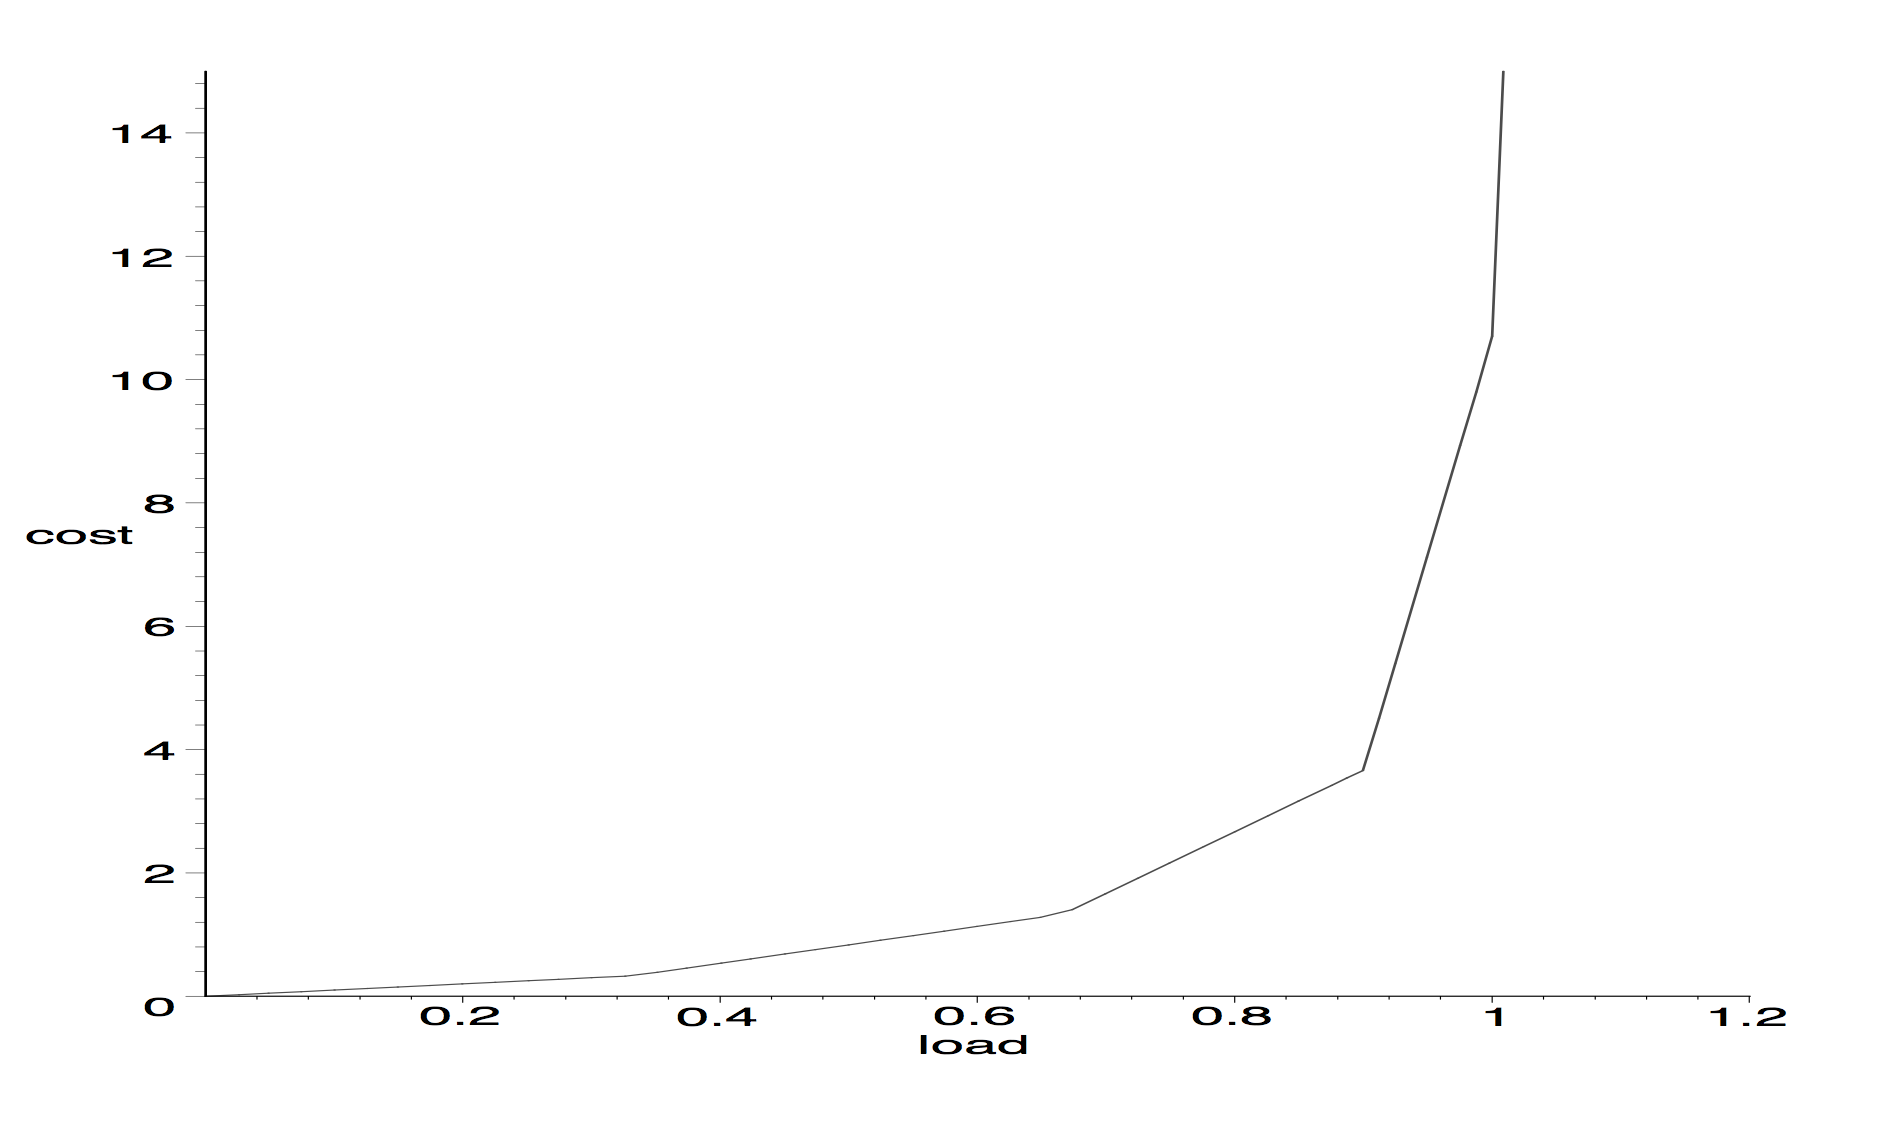
\includegraphics[scale=0.90]{piecewise.png} 
 
 We can apply the same piecewise linear function for node utilization, and the objective function could be minimize 
 $\Phi_e + \Phi_v$.

\subsection{Resource Allocation for a Given Network} All previous LP formulations are all assuming link capacity and node capacity B(e) and C(v) are all fixed, but in fact those could be variables; the objective can be to minimize the hardware cost while keeping utilization for each link and node low, without losing generality, we focus on optimizing node processing capacity placement C(v) since it is closer to reality where we have a relatively fixed topology with node capacity reassignment can happen at daily base. In fact B(e) can be derived through the same mechanism. 
\begin{subequations}
\begin{align*}
&\forall v; 0 \leq C(v) \leq max(v) ,\\
&\forall v; u(v) \leq \beta
\end{align*}
\end{subequations}
Here $\beta$ could be the load for middleboxes $\in (0,1)$ the networking operation tries to achieve and it is tunable.

Here the objective function could be as simple as, saying minimize the total hardware cost for middlebox plus routing cost; or in math interpretation  $minimize \sum\limits_v C(v)+ \sum\limits_e \Phi_e$.  

There is one more thing to capture in allocation: so far we assume each network flow is static and prefixed, but traffic pattern actually changes over time. To solve this solution, we can use either Stochastic Linear Programming or Robust Optimization. In networking setting, RO seems like a better choice since SLP tends to give us better value for the objective, it is harder to maintain stability over all scenarios and have higher cost to adjust to changes. Furthermore, SLP tries to satisfy all constraints and simply declare infeasible if failed to meet that goal. Networking design are usually conservative and people are willing to pay a little higher cost to ensure the system being able to keep up with changing demands, and feasible solution with heavy penalty is preferred over infeasible solution.

Let us review the LP formulation:
 
Objective: Minimize $\sum\limits_v C(v)+ \sum\limits_e \Phi_e$

Subject to:
\begin{subequations}
\begin{align}
&\forall v \in V-\{s, t\}; \sum\limits_i \sum\limits_{in}  f_i(e)= \sum\limits_i  \sum\limits_{out} f_i(e),\\
&\forall e, i; 0 \leq w_i(e) \leq f_i(e),\\
&\forall v, i; p_i(v) =  \sum\limits_{in } w_i(e) -  \sum\limits_{out} w_i(e) ;\\
&\forall v; p_i(v)\geq 0 ,\\
&\forall v; \sum\limits_i p_i(v)\leq \beta*C(v),\\
&\forall e\in(s, v) ; w_i(e) =f_i(e),\\
&\forall e\in(v, t) ; w_i(e) =0,\\
&\forall e\in(s, v) ; \sum\limits_v f_i(s,v) =D_i.
\end{align}
\end{subequations}
We have a set of $D_i$'s which can be provided through continuous measurement, i.e. we have flow demand from time t=1 to T, $D^{1:T}$. Each $D^{t} = \{D_1^t, \dots, D_i^t\}$ are essentially control variables. C(v)'s are design variables, we would fix it in various input settings. Other variables such as $p_i(v)$ are coefficients of input $D_i$, and therefore we can relax 6.10e with an error vector: $\sum\limits_i p_i(v)- \beta*C(v) =z(v)$. 

In RO it has a certain probability for each input $D^t$, and here for simplicity it can be modeled as uniform, i.e. each $p_t=\frac{1}{T}$.
New objective function is Minimize $ \bar{ \xi} + \lambda *\sigma + \omega*\epsilon  $.
\newline
$\xi_t= \sum\limits_v C(v)+ \sum\limits_e \Phi^t_e$ is the cost function for each input $D^t$\.\newline
$\lambda$ and $\omega$ are two sensitive parameters for  $\sigma$ as deviation cost and $\epsilon$ error cost.\newline
Previously people have used both sum of squares and sum of absolute values to capture the cost of changes, and some work shows that using sum of absolute values are more robust than sum of squares, so here we apply sum of absolute values, it also perfectly conserves the LP format. \newline
$\sigma = \frac{ \sum\limits_t  |\xi_t- \bar{\xi}|}{T}$\newline
$\epsilon= \frac {\sum\limits_t (\sum\limits_v |z_t(v)|)}{T}$

To make LP better fit in networking setting, we again can apply linear piecewise error cost functions.
$
cost(z )=
\left\{
	\begin{array}{ll}
		0  & \mbox{if } z\leq 0 \\
		z & \mbox{if } z > 0 
	\end{array}
\right.
$\newline
Furthermore, we can also segment the node utilization into three ranges: $[0, \beta^1); [\beta^1, \beta^2]; (\beta^2, + \infty)$, here we have $z^1 = \beta^1*C(v)-\sum\limits_i p_i(v) $ and $z^2 =\sum\limits_i p_i(v) -\beta^2*C(v) $, e.g. set $\beta^1 = 0.5$ and $\beta^2 = 0.9$, therefore we can penalize both under-utilization and over-utilization. Here we decide to use absolute value instead of scalar for error vector $z$ is due to preserving LP format. 




%%%%%%%%%%%%%%%%%%%%%%%%%%%%%%%%%%%%%%%
%%%%%%%%%%%%%%%%%%%%%%%%%%%%%%%%%%%%%%%
%%%%%%%%%%%%%%%%%%%%%%%%%%%%%%%%%%%%%%%
%%%%%%%%%%                      After Main Text                 %%%%%%%%%%
%%%%%%%%%%%%%%%%%%%%%%%%%%%%%%%%%%%%%%%
%%%%%%%%%%%%%%%%%%%%%%%%%%%%%%%%%%%%%%%
%%%%%%%%%%%%%%%%%%%%%%%%%%%%%%%%%%%%%%%

\bibliographystyle{acm}

\bibliography{references}

\appendix
%%%%%%%%%%%%%%%%%%%%%%%%%%%%%%%%%%%%%%%%
%%%%%%                            Equivalence                      %%%%%%%%%%%
%%%%%%%%%%%%%%%%%%%%%%%%%%%%%%%%%%%%%%%%
\section{Proof for edge based LP for section2.1}
Unlike a simple max flow model this is not very intuitive that our LP formulation is feasible to realize it in path based solution; e.g. it is not easy to find a path to guarantee both link capacity and processing capacity. To achieve it, we need to show two directions:
\begin{itemize}
  \item {\textit{Direction A:} If there is a path-based LP solution, we have an edge-based requirement fulfilled.}
  \item {\textit{Direction B:} If there is an edge-based LP solution, we have a path-based solution.}
\end{itemize}
For \textbf{\textit{Direction A}}, it is easy to show. Once we get a path based solution, we sum up the path-based solution and put it together to a edge-based solution. Through the proof we are using f/w representation for edge-based formulation.

\begin{proof}

For each edge e, $f(e) =\sum\limits_{\pi\in P: e\in \pi} f(\pi)$.

For each node v, $w(e) = \sum\limits_{\pi\in P: e'\in \pi, e' <<= e} w(\pi, e')$ ($<<=$ means e' is topologically at or after e on the path).

Since flow is built based on path, we have $ \sum\limits_{(u,v)\in E} f(e) $=$ \sum\limits_{\pi\in P, v\in \pi} f(\pi)$ = $\sum\limits_{(v,w )\in E} f(e)$.

For each path we also have:

$w(e) =$ 
$ \sum\limits_{\pi\in P: e'\in \pi, e' \leq e} w(\pi, e')\leq \sum\limits_{\pi\in P: e\in \pi} f(\pi) = f(e).  $\newline
\end{proof}
\fbox{ \includegraphics[scale=0.63]{algo1.png} }
\fbox{ \includegraphics[scale=0.63]{algo2.png}}
   
Next we focus on proof for \textbf{\textit{Direction B}}.

That is, if we have a solution which tells us that if we can assign certain amount of flow and processing 
demand at each edge, we are able to construct paths with a certain amount of flow 
and corresponding processing demand and process workload at every/some node along the path in a certain way.


Setup:
A set of nodes  v$\in$ V, a set of edges e(u,v)$\in$ E. We have the solution of from edge-based LP, with 
f(e) is the flow for each edge and w(e) is workload demand at that edge. We also have processing work at each node p(v) and it is simply $p(v) = 
\sum\limits_{e \in E_{u, v} }w_(e) - \sum\limits_{e \in E_{v, w} }w_(e)  $.

We first build a graph with all vertices \textit{V}, and for $\forall e(u,v) \in E $, if f(e)$ >$0, we put a direct edge e(u,v) in the graph. We might have cycles or even two flows with opposite directions at the same edge. Then we run algorithm [Path Construction] to get one path to allocate flow. For each flow path, we run flow allocation and update the graph, we exhaustively do it until we place all flow and workload demand, this step is essentially captured in algorithm [Flow Placement]. 

We need to prove from two sides for this algorithm: 
\begin{itemize}
  \item {Side 1: there is p(v) >0, we can always find a path with non-zero flow}
   \item {Side 2: after allocation for one path, constraints are held for the reduced graph} 
\newline
\end{itemize}
Here we introduce an variable $\rho$ for each edge e where $\rho_{e} = \frac{ w(e)}{f(e)}$.
\begin{lemma}
If there is a cycle, we always have one incoming edge with $\rho =1$ and outgoing edge with $\rho =0$ at cross point.
\end{lemma}
\begin{proof}
If we think this in a $f^1/f^2$ way, $\rho = \frac{ f^1} {f^1+f^2 }$. Here since $f^2=0$ for incoming edge based on lemma2.2, we have $\rho=1$. The same way to get $\rho_{out}=0$ since $f^1=0$ for outgoing edge. 
\end{proof}

\begin{theorem}Our path composition can always generate path with non-zero flow from source to sink. \end{theorem}
\begin{proof}
\textit{First}, based on lemmaA.1, we can split the $cross\text{ } node$ into two nodes while preserving the links, and the traversal at two augmented nodes will pick different incoming and outgoing links due to relations of $\rho$'s  in the algorithm, so we never pick the same node twice if we think about forward or backward traversal along, although the two directions may meet at some node(s) along the traversal, and thus it is effectively a DAG. For a DAG we can always reach source and sink.

\textit{Second} we need to show for a certain path $\exists e; w(\pi, e)>0$. Since $\delta = min( p(v),$ $w(e_{i}),f(\pi) -w(\pi,e_{i+1}))$; at node v where $p(v)>0$; we have $w(e_i)>0$ because $[\rho_{in} =\frac{ w(e_{in})}{f(e_{in})} ]>\rho_{out}\geq 0$. If $\delta=0$ we have $ f(\pi) -w(\pi,e_{i+1}) =0$, which lead to $ w(\pi, e_{i+1})>0$, otherwise $ \delta>0;w(\pi, e_i) = [ \delta+w(\pi, e_{i+1} )]>0$.

\textit{Finally} our algorithm by design conserve the flow and ensures workload demand is decreasing since w is using backward greedy algorithm.
\end{proof}

This essentially proves \textbf{Side 1}.

\begin{theorem}Flow placement algorithm conserves all the constraints for the reduced graph.
\end{theorem}
\begin{proof}
for 2.1a:\newline
$\forall v \in \pi; \sum\limits_{in}  f(e) - \sum\limits_{out} f(e)$=
\newline$\sum\limits_{in \not=e_i}  f(e) - \sum\limits_{out\not=e_{i+1} } f(e) +[f(e_i)-f(\pi) ] - [f(e_{i+1}) -f(\pi)] = 0 $
\newline
2.1b\newline
$ \forall e \in \pi; f(e) = f(e)-f(\pi) \geq f(e)-f(e) \geq 0$\newline
2.1c\newline
$\forall e \in \pi; f(e) = f(e)-f(\pi) \leq B(e)-f(\pi)=B^{new}(e)$\newline
2.1d\newline
$\forall e \in \pi; w(e) = w(e) - w(\pi, e) \geq w(e) -w(e) \geq 0$\newline
2.1e\newline
$\forall e \in\pi; f(\pi, e)-w(\pi, e) \leq f(e) -w(e) =>w(e) -w(\pi, e) \leq f(e) -f(\pi, e) $\newline
2.1f\newline
$\forall v \in \pi; p(v) = p(v) -\delta \geq p(v) -p(v) \geq 0 $\newline
2.1g\newline
$\forall v \in \pi; p(v) - \delta \leq C(v) - \delta $\newline
2.1h and 2.1i are ensured by greedy algorithm, $w(\pi, e_1) = f(\pi) $ and $w(\pi, e_k)=0$.
\end{proof}
This essentially proves \textbf{Side 2}.

\section{Proof for edge-based solution for Section 4}
For this part, we need to rewrite the path based solution so it is easier to understand, and also easier to be mapped from section 4 LP. Here again we assume the traffic change rate is r, e.g. if we convert $ f^1$ traffic at node v, we have $r*f^1$ traffic generated. Here again we use $f^1(\pi, e) /f^2(\pi, e)$ to represent the unprocessed and processed flow at edge e on path $\pi$.

Objective: Maximize  $\sum \limits_{\pi\in P} f(\pi) $
\newline

Subject to:
\newline
\begin{subequations}
\begin{align}
&\forall e, \pi;  f^1(\pi, e) +f^2(\pi, e)/r= f(\pi),\\
&\forall e; \sum \limits_{\pi\in P:e\in \pi} f(\pi) \leq B(e),\\
&\forall  v; \sum \limits_{\pi\in P} \sum \limits_{ e,e'\in \pi} f^1(\pi, e) -f^1(\pi, e')\leq C(v),\\
& where \;(e, e') = (u,v)->(v,w).\nonumber\\
&\forall  v; \sum \limits_{ e,e'\in \pi} f^1(\pi, e) -f^1(\pi, e')\geq 0,\\
& where \;(e, e') = (u,v)->(v,w).\nonumber\\
&\forall e; f^2(\pi,e)\geq 0, \\
&\forall e; f^1(\pi,e)\geq 0, \\
&f^2(\pi,(s,v))= 0, \\
&f^1(\pi, (w,t)) =0, 
\end{align}
\end{subequations}
Again we introduce some intermediate variable p for each node, $p_v: $ workload processed at node v.
\newline
$p_v = \sum\limits_{e \in E_{u, v} } f^1(e) - \sum\limits_{e \in E_{v, w} } f^1(e)  $ .
\newline
\fbox{ \includegraphics[scale=0.60]{algo3.png} }
\fbox{ \includegraphics[scale=0.62]{algo4.png}}
   
The proof for showing this is feasible in path-based solution from an edge-based solution is similar to proof above. 
Again we can verify that we can always ensure some path with non-zero flow from source to sink, and also all the constraints are conserved after peeling off some path. 
\begin{theorem}Our path composition can always generate path with non-zero flow from source to sink. \end{theorem}
\begin{proof}
\textit{First} we can still use lemma 2.1 and lemma A.1 to show that the graph is effectively a DAG, so we can always reach destination from source through our path construction.
\textit{Second} we need to show for a certain path $\exists e; f(\pi)>0$. Since $\delta = min( p(v),f^1(\hat{e}),f^2(\bar{e'}))$; at node v where $p(v)>0$; we have $f^1(e_i)>0$ because $[\rho_{in} =\frac{ f^1(e_{in})}{f^1(e_{in})+f^2(e_{in})/r} ]>\rho_{out}\geq 0$. Since we keep picking max $\rho$ for upstream nodes, they must have $f^1>0 $ for any edge we choose as sum of incoming $f^1$ from any node must be greater or equal to sum of outgoing $f^1$. For downstream, essentially we are pick max $\rho_2 = 1-\rho$, and the same proof for $f^2$. So we must have non zero flow at this path.

\textit{Finally} our algorithm by design conserve the flow and ensures unprocessed flow $f^1$ is decreasing since $f^1$ is using backward greedy algorithm.
\end{proof}

\begin{theorem}Flow placement algorithm conserves all the constraints for the reduced graph.
\end{theorem}
\begin{proof}
4.4a:\newline
$\forall v \in V-{s, t}; \sum\limits_{in} ( r* f^2(e) +f^1(e)) - \sum\limits_{out } (r*f^2(e) + f^1(e)) =\sum\limits_{in\not=e_i}[f^1(e) +r*f^2(e)] - \sum\limits_{out\not=e_{i+1} } [f^1(e)+r*f^2(e)] +[f^1(e_i)+f^2(e_i)*r-f^1(\pi, e_i) - r*f^2(\pi, e_i) ] - [f^1(e_{i+1})+f^2(e_{i+1})*r -f^1(\pi, e_i) - r*f^2(\pi, e_i) ] = f(\pi)*r - f(\pi)*r =0  $
\newline
4.4b\newline
$\forall e \in \pi; f^2(e) = f^2(e) -f^2(\pi, e) \geq f^2(e) -min(f^2(e)) \geq 0$  
\newline
4.4c:\newline
$\forall e \in \pi; f^1(e) = f^1(e) -f^1(\pi, e) \geq f^1(e) -min( f^1(e) )\geq 0$;\newline
4.4d\newline
$\forall e \in \pi; f^1(e) +f^2(e) = f^1(e)-f^1(\pi, e) +f^2(e)- f^2(\pi, e) \leq B(e)- f^1(\pi, e) - f^2(\pi, e) .$
\newline
4.4e\newline
$\forall v \in \pi; \sum\limits_{in } f^1(e) - \sum\limits_{out} f^1(e) = \sum\limits_{in } f^1_{old}(e) - \sum\limits_{out} f^1_{old}(e) -\delta= p(v) -\delta \geq 0$\newline
4.4f\newline
$\forall v \in \pi; \sum\limits_{in } f^1(e) - \sum\limits_{out} f^1(e) = \sum\limits_{in } f^1_{old}(e) - \sum\limits_{out} f^1_{old}(e) -\delta= p(v) -\delta \leq C_{old}(v) -\delta$\newline
4.4g, 4.4h are correct by value assignment, we assign $f^1(\pi,(w, t) )=0$ so $f^1(w, t) =0$ is conserved, and $f^1(\pi, (s, v)) =f(\pi) => f^2(\pi, (s,v)) =0$ so $f^2(s, v)=0$ is conserved. 
\newline
\end{proof}

\section{Proof for Multitask Flow}
\subsection{Sequential}
First let us rewrite the LP, again we use the different flow formulation, which means there are three different flows here, they are preprocessed, post a but pre b processed, and post b processed.

Objective: Maximize $\sum \limits_{v: (s, v) \in E} f^1(e) $ 

Subject to:
\begin{subequations}
\begin{align}
&\sum\limits_{in} ( f^2(e)+ f^1(e) +f^3(e)) \nonumber\\
&= \sum\limits_{out } ( f^2(e)+ f^1(e)+f^3(e))\\
&for\; \forall v \in V-\{s, t\}; \nonumber\\
&\forall e; f^3(e)\geq 0,\\
&\forall e; f^2(e)\geq 0,\\
&\forall e; f^1(e)\geq 0,\\
&\forall e; f^1(e)+ f^2(e) + f^3(e)\leq B(e),\\
&\forall v; p_a(v) = \sum\limits_{in } f^1(e) - \sum\limits_{out} f^1(e) \\
&\forall v; p_b(v) = \sum\limits_{out } f^3(e) - \sum\limits_{in} f^3(e) \\
&\forall v;p_a(v)\geq 0, \\
&\forall v;p_a(v)\leq C_a(v),\\
&\forall v;p_b(v)\geq 0, \\
&\forall v;p_b(v)\leq C_b(v),\\
&\forall e\in (s,v); f^2=0, \\
&\forall e\in (s,v); f^3=0, \\
&\forall e\in (v,t); f^1=0,\\
&\forall e\in (v,t); f^2=0.
\end{align}
\end{subequations}

We also write down the edge based formulation:

Objective: Maximize  $\sum \limits_{\pi\in P} f(\pi) $
\newline

Subject to:
\newline
\begin{subequations}
\begin{align}
&\forall e, \pi;  f^1(\pi, e) +f^2(\pi, e)+ f^3(\pi, e)= f(\pi),\\
&\forall e; \sum \limits_{\pi\in P:e\in \pi} f(\pi) \leq B(e),\\
&\forall  v; \sum \limits_{\pi\in P} \sum \limits_{ e,e'\in \pi} f^1(\pi, e) -f^1(\pi, e')\leq C_a(v),\\
& where \;(e, e') = (u,v)->(v,w).\nonumber\\
&\forall  v; \sum \limits_{ e,e'\in \pi} f^1(\pi, e) -f^1(\pi, e')\geq 0,\\
& where \;(e, e') = (u,v)->(v,w).\nonumber\\
&\forall  v; \sum \limits_{\pi\in P} \sum \limits_{ e,e'\in \pi} f^3(\pi, e') -f^3(\pi, e)\leq C_b(v),\\
& where \;(e, e') = (u,v)->(v,w).\nonumber\\
&\forall  v; \sum \limits_{ e,e'\in \pi} f^3(\pi, e') -f^3(\pi, e)\geq 0,\\
& where \;(e, e') = (u,v)->(v,w).\nonumber\\
&\forall e; f^1(\pi,e)\geq 0, \\
&\forall e; f^2(\pi,e)\geq 0, \\
&\forall e; f^3(\pi,e)\geq 0, \\
&f^2(\pi,(s,v))= 0, \\
&f^3(\pi,(s,v))= 0, \\
&f^1(\pi, (w,t)) =0, \\
&f^2(\pi, (w,t)) =0.
\end{align}
\end{subequations}

Again $f^1; f^2; f^3$ are three different types of flows which represents pre processed, post a processed but pre b processed, and post b processed. Again we can make some observation for the paths:

\begin{lemma}
If there is cycle(s) on the path, there must be $f^1=0 $ for outgoing edge and $f^3=0$ for incoming edge. 
\end{lemma}

\begin{proof}
Apply the same flow cancellation method, since unprocessed flow are "detoured" to be processed, and if there is no process happening in the cycle, we can simply cancel the $f^1$ part with no side effect.

The same mechanism for $f^3$. A fully processed flow (after both a and b process) does not need to be trapped in a cycle, as we can cancel $f^3$ with no side effect. 

Since $f^1$ is always decreasing while $f^3$ is always increasing, so incoming edge has $f^3=0$ and outgoing edge has $f^1=0$ in the cycle.
\end{proof}

Here we introduce two intermediate variables $\rho_1 = \frac{f^1} {f^1+f^2+f^3}$ and $\rho_3 = \frac{f^3} {f^1+f^2+f^3}$ for each edge. 
\fbox{ \includegraphics[scale=0.64]{algo5.png} }
\begin{lemma}
Path construction always give us non zero path from source to destination. 
\end{lemma}
\begin{proof}
First case if at node v where $p_a(v)>0$, $p_b(v)$ is also non zero, or in other words, v=v', so it must have non zero $f^1$ coming in and non zero $f^3$ going out, since we keep picking max $\rho_1 $ and $\rho_3$, we will get non zero value from source to destination.

Second case if at node v where $p_a(v)>0$, $p_b(v)=0$, so we must have $f^2>0$ coming out from node v, and if we keep picking $f^2>0$ via BFS, we will find some node v' where $p_b(v')>0$, we can again disqualify the existence of cycles where $f^2>0$ from outgoing edges in the cycle by flow cancellation. Once we find the node v', the rest is the same as above.  
\end{proof}
\fbox{ \includegraphics[scale=0.64]{algo6.png} }

Again here is not hard to find that all the constraints are preserved after flow placement, so the algorithm will keep peeling off flow from edge based solution and construct paths, until no $p_a(v) $ left, which also means no $p_b(v)$ left. 
%%%%%%%%%                                        Parallel                  %%%%%%%%%%%%%%%%%%%%%
\subsection{Parallel}
let us again rewrite the LP using the different flow formulation, which means there are four different flows here, they are preprocessed $f^1$, post a but pre b processed $f^2$, post b but pre a processed $f^3$, and post a and b processed $f^4$.

Objective: Maximize $\sum \limits_{v: (s, v) \in E} f^1(e) $ 

Subject to:
\begin{subequations}
\begin{align*}
&\sum\limits_{in} ( f^2(e)+ f^1(e) +f^3(e)+f^4(e)) \nonumber\\
&= \sum\limits_{out } ( f^2(e)+ f^1(e)+f^3(e) + f^4(e))\\
&for\; \forall v \in V-\{s, t\}; \nonumber\\
&\forall e; f^4(e)\geq 0,\\
&\forall e; f^3(e)\geq 0,\\
&\forall e; f^2(e)\geq 0,\\
&\forall e; f^1(e)\geq 0,\\
&\forall e; f^1(e)+ f^2(e) + f^3(e) + f^4(e)\leq B(e),\\
&\forall v; p_a(v) =\nonumber\\
& \sum\limits_{out } (f^2(e)+f^4(e)) - \sum\limits_{in} (f^2(e)+f^4(e)); \\
&\forall v; p_b(v) = \nonumber\\
&\sum\limits_{out }( f^3(e) +f^4(e)) - \sum\limits_{in}( f^3(e) +f^4(e));\\
&\forall v;p_a(v)\geq 0, \\
&\forall v;p_a(v)\leq C_a(v),\\
&\forall v;p_b(v)\geq 0, \\
&\forall v;p_b(v)\leq C_b(v),\\
&\forall e\in (s,v); f^2=0, \\
&\forall e\in (s,v); f^3=0, \\
&\forall e\in (s,v); f^4=0, \\
&\forall e\in (v,t); f^1=0,\\
&\forall e\in (v,t); f^2=0,\\
&\forall e\in (v,t); f^3=0.
\end{align*}
\end{subequations}

This LP formulation is can be interpreted as two previous LPs with sequentially a before b and b before a, the same path construction except we have to consider process b could either happen before or after process a, and it can be proved via the same methods. 




\end{document}

% End of ltexpprt.tex